
%%
\documentclass[preprint,12pt]{elsarticle}
\usepackage[left=2cm, right=5cm, top=2cm]{geometry}


%% The graphicx package provides the includegraphics command.
\usepackage{graphicx}
%% The amssymb package provides various useful mathematical symbols
\usepackage{amssymb}
\usepackage{amsfonts}
\usepackage{tikz}
%% The amsthm package provides extended theorem environments
%% \usepackage{amsthm}

%% The lineno packages adds line numbers. Start line numbering with
%% \begin{linenumbers}, end it with \end{linenumbers}. Or switch it on
%% for the whole article with \linenumbers after \end{frontmatter}.
\usepackage{lineno}
\usepackage{seqsplit}
\usepackage[nottoc]{tocbibind} 


% \biboptions{}

\journal{Part C Dissertation Oxford University}
\begin{document}

\begin{frontmatter}

%% Title, authors and addresses

\title{Extensions of number fields with small ramification}



\author{Samuel Bodansky}

\address{Oxford,UK}

\begin{abstract}
Aim: to construct minimally ramified extensions of number fields.
\end{abstract}
\end{frontmatter}
\section{Notation}
\begin{enumerate}
    \item K is a number field, h(K) is its class number and Cl(K) is its ideal class group.
    \item $d_K$ is the discriminant of K.
    \item $K^{ur}$ is the maximally unramified extension of K.
    \item $n_K$ is the degree of the extension $K:\mathbb{Q}$.
    \item KL denotes the compositum of two number fields K and L.
    \item $rd_K$ is the root discriminant of K, $|d_K|^\frac{1}{n_K}$ .
    \item $G_K$ is the Galois group $\Gamma(\bar{K}:K)$
    \item $G_K^{ur}$ is the Galois group $\Gamma(K^{ur}:K)$
    \item $C_K$ is the class field group of K. 
    \item $G^{ab}$ is the abelianisation of a group G, $G/[G,G]$
    \item $K_n$ is the $n_{th}$ term in the sequence defined by $K_0:=K$ and $K_{n+1}$ is the Hilbert class field of $K_n$.
    \item $\zeta_n$ is the $n_{th}$ root of unity. 
\end{enumerate}
\section{Summary of Relevant Literature}
\subsection{Jones and Roberts}

\section{Initial Results}
\subsection{Goal and Background}

Recall a prime ideal $\mathfrak{p}$ in $\mathcal{O}_K$ factors in an extension L of K as
\newline
$\mathfrak{p}\mathcal{O}_L=\mathfrak{B}_1^{e_1}...\mathfrak{B}_m^{e_m}$ where $\mathfrak{B}_i$ are ideals in $\mathcal{O}_L$ intersecting $\mathcal{O}_K$ at $\mathfrak{p}$. Each $e_i\geq1$ and if $e_i>1$ for some i then we say that $\mathfrak{p}$ ramifies in L. If $e_i=1$ for all i then we say $\mathfrak{p}$ splits in L.
\newline
When L is a Galois extension of K, all of the $e_i$ are equal and in fact split(L:K) determines L.
\newline
In fact, if the set of primes that split in L and $\tilde{L}$ then algebraic number theory can show that $split(L:K)=split(L\tilde{L}:K)=split(\tilde{L}:K)$ and indeed $[L:K]=[L\tilde{L}:K]=[\tilde{L}:K]$. 
\newline
A natural question is to determine these sets split(L:K) as L changes over the finite extensions of K, and to determine the sets L corresponding to these extensions.
\newline
Let H be a subgroup of the class group C of K. A finite unramified abelian extension L of K is said to be a $\textit{class field}$ for H if the prime ideals of K splitting in L are exactly those in $\tilde{H}$ . The following theorem provides an answer the above question for unramified abelian extensions of K.
\newline
Theorem: A class field exists for each subgroup of C; it is unique, and every finite unramified abelian extension of K is the class group of some subgroup of C. If L is the class field of H, then $\Gamma(L/K)\cong C/H$ and for every prime ideal $\mathfrak{p}$ of K, $f(\mathfrak{p})$ is the order of the image of $\mathfrak{p}$ in the group C/H.
\newline
The class field of the trivial subgroup of C is called the Hilbert class field of K. It isthe largest abelian extension, L of K unramified at all primes of K.
\newline
For example,if $K=\mathbb{Q}[\sqrt{-5}]$ then take $L=\mathbb{Q}[\sqrt{-1},\sqrt{-5}]$. L is an unramified degree 2 extension of K and so the Hilbert class field of K is $K[\sqrt{-1}]$.

\subsection{First results}
Goal: For a given number field K, what is the maximal unramified extension $K^{ur}$ of K is and also what is the structure of $G_K^{ur}$ is. By Class Field Theory we already know that 
\[(G_K^{ur})^{ab} = \Gamma(K_1:K)\cong C_K\].
\newline
\subsection{Important Results from Class Field Theory}
1. \cite{YAMA}[Proposition 1] gives the following classification of polynomials of the form $f(x) = x^n+ax+b \in \mathbb{Z}[x]$, and K is the splitting field of f over $\mathbb{Q}$.
\newline
If the following conditions hold:
\begin{enumerate}
    \item (n-1)a and nb are relatively prime 
    \item $\Gamma(K/\mathbb{Q}) \cong S_n$
\end{enumerate}
\newline
Then K is an $A_n$-extension of $\mathbb{Q}(\sqrt{\Delta(f)})$ which is unramified at all finite primes. For example, if $f(x) = x^5-x+1$, then $\Delta(f)= 2869$ and write $L = \mathhbb{Q}(\sqrt{2869})$. Then K is unramified over L and $\Gamma(K:L)\cong A_5.$

\subsection{Bounds on Discriminants}
Minkowski's theorem bound shows that if K is a number field with $r_1$ real and $2*r_2$ complex conjugate fields, and $n=r_1+2r_2$ is the degree of the field, then 
\newline 
\[rd_K\geqslant (\frac{\pi}{4})^{\frac{2r_1}{n}}\frac{n^2}{n!^{\frac{2}{n}}}\]
\newline
As $n\rightarrow \infty$, Stirling's formula can give a bound that $rd_K\geqslant e^2 = 7.39$.
\newline
Odlyzko's Bound \cite{ODL2} improved on the bounds for Minkowski for the discriminant of a number field. It can be stated as  
\medskip
\newline
\[rd_K\geqslant 60^{(\frac{r_1}{n})}22^{(\frac{r_2}{n})}+o(1)\] as $n\rightarrow \infty$.
\newline
Furthermore, under the assumption of the Generalised Riemann Hypothesis, 
this bound can be improved by replacing the numbers 60 and 22 by 188 and 41 respectively. 
\subsection{How to use this bound}
Following \cite{YAMA}, write this bound function as $B(n,r_1,r_2)$, and let H be a positive integer. Suppose that L is an unramified normal extension of K of degree M. Then if
\newline{}
(i) $rd_K<B(H.m.n,H.m.r_1,H.m.r_2)$ then $[K^{ur}:L]<H$ and $h(L)<H$. Indeed if H=2 then $K^{ur}=L$.
\newline
(ii) If h(L)=1 and H=60 then again $K^{ur}=L$.
\subsection{Result using Hoelscher}

Using \cite{HOEL} and \cite{JONE}, we see that 
the prime p=239 is tamely ramified for \[G=S_3,G\textsuperscript{ab} = 2, p_w =3  \] and also 
\newline
\[G=D_5,G\textsuperscript{ab} = 2 \]
This means that we can apply Theorem(1.1) from Hoelscher with \[N = G = D_5, K_0 = \mathbb{Q}\]
\newline
Then \[N/p(N) = D_5 \not\subset \mathbb{Z}/(p-1) = \mathbb{Z}_{238}\]
\newline
We have the field extension diagram
\bigskip
\newline
\begin{center}
    
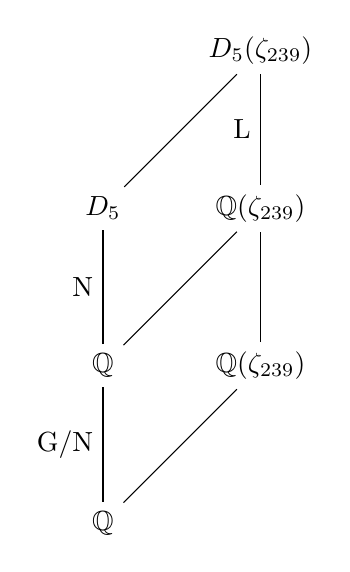
\begin{tikzpicture}[node distance = 2cm, auto]
      \node (Q) {$\mathbb{Q}$};
      \node (K0) [above of=Q] {$\mathbb{Q}$};
       \node (QZP) [above of=Q, right of=Q] {$\mathbb{Q}(\zeta_{239})$};
       \node (K) [above of=K0] {$D_5$};
       \node (K0ZP) [above of=QZP] {$\mathbb{Q}(\zeta_{239})$};
       \node (KZP) [above of=K0ZP] {$D_5(\zeta_{239})$};
       
       \draw[-] (Q) to node {G/N} (K0);
       \draw[-] (K0) to node {N} (K);
       \draw[-] (K) to node {} (KZP);
       \draw[-] (K0ZP) to node {L} (KZP);
       \draw[-] (QZP) to node {} (K0ZP);
       \draw[-] (Q) to node {} (QZP);
       \draw[-] (K0) to node {} (K0ZP);
      \end{tikzpicture}
\end{center}
\newline
Where the field extension L is a non-trivial abelian unrafimifed sub-extension of degree prime to p with L Galois over $\mathbb{Q}$.
\subsection{Maire's Results for infinite non Galois unramified extension}
Following from \cite{MAIR}[5.1], there exist infinitely many quadratic fields with a finite 2-Hilbert tower, but having an infinite ramified extension of $2^{\infty{}}$. 
The following methodology was implemented  to find suitable polynomials:
\newline
\begin{enumerate}
    \item Pick 8 real numbers close to 0 and define $\tilde{P}(x)$ to be the polynomial with these roots. This is done to increase the probability that P(x) will also have 8 real roots. 
    \item Find a polynomial P(x) which is near to $\tilde{P}(x)$.
    \item Check that the P(x) is irreducible, has 8 real roots and has prime discriminant. 
    \item Search for primes 3 mod 4 which totally decompose in the splitting field of P. 
\end{enumerate}
The following polynomial was found: 
\newline
$P(X) = (x^8 - 3x^7 - 16x^6 + 31x^5 + 74x^4 - 40x^3 - 56x^2 + 17x + 3)$,
where 
\newline
$l = \Delta(P) = 76363470193820546413$. 
\newline
Put $q_1 = 219823$, $q_2 = 931363$, $K = split(P, \mathbb{Z}[x])$.
\newline
Here $q_1$ and  $q_2$ are totally decomposed in $K/\mathbb{Q}$, the Galois closure of P.
\newline
Use the following definitions: 
\begin{itemize}
    \item $N = K\mathbb{Q}(\sqrt{l})$. Note $q_1$ and $q_2$ decompose completely in $N/\mathbb{Q}$, an extension of degree 16.
    \item $E = N(\sqrt{q_1*q_2})$
    \item $E_2$ is the infinite 2-Hilbert tower of E.
\end{itemize}
\newline 
We can now draw the following field diagram, where all extensions are unramified 2-extensions. 

\begin{center}
    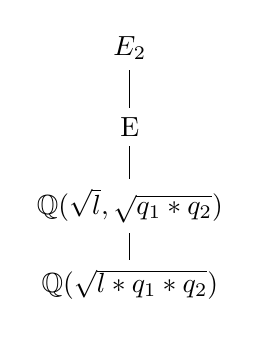
\begin{tikzpicture}[node distance = 1cm, auto]
      \node (Q12) {$\mathbb{Q}(\sqrt{l*q_1*q_2})$};
      \node (QL12) [above of=Q12] {$\mathbb{Q}(\sqrt{l},\sqrt{q_1*q_2})$};
      \node (E) [above of=QL12] {E};
      \node (E2) [above of=E] {$E_2$};
      \draw [-] (Q12) to node {} (QL12);
      \draw [-] (QL12) to node {} (E);
      \draw [-] (E) to node {} (E2);
      \end{tikzpicture}
\end{center}
\newline
In fact, $E_2/\mathbb{Q}(\sqrt{l*q_1*q_2})$ is an unramified field extension of degree $2^{\infty}$.



\section{Trying to recreate Maire's Results}
In \cite{MAIR}[3.1] I use Maire's method to find a suitable polynomial. 
Using SYMPY I found the following polynomial:
\newline
\begin{equation*}\label{eq:soln mle2}
  \begin{aligned}
(x - 306678861179996894)^{2}(x - 157643009028967297)
(x - 26634967141504290)(x + 28702432430906831)(x + 379563374979692451)(x +389369891119866095)
 \end{aligned}
\end{equation*}
\newline
with discriminant $l = \Delta(P) = 1486256555685463501$.
\newline
\cite{MAIR}[2.1] gives a condition for the p-Hilbert tower of K to be infinite. 
\newline
\cite{MAIR}[2.3] says that if P is an irreducible polynomial in $\mathbb{R}[x]$ with squarefree discriminant D(P), and C is its Galois closure, then $C/\mathbb{Q}(\sqrt{\Delta(P)})$ is unramified.
\newline
Using these two propositions from Maire can give an algorithm to find a field $K=\mathbb{Q}(\sqrt{l_1.l_2.l_3)}$, where $l_1$ is a prime 1 modulo 4, and $l_2$ and $l_3$ are primes 3 modulo 4. 
\newline
Here is an example for n= 5:
$(x^5 + 12x^4 + 20x^3 - 96x^2 - 4399, D=1255760665676742389)$


\label{S:2}
\subsection{Subsection Three}
\section{Using Sympy to find Maximal Unramified Extensions}
Here is an algorithm to find the maximal unramified extension of a number field using Odlyzko's bound and result from Kim \& Koenig and Maire.
\begin{enumerate}
  \item  Order the irreducible quintic polynomial in $\mathbb{Z}[x]$ by the absolute value of their discriminant. 
  \item Pick f(x) to be a possible quintic polynomial.
  \item Calculate $\Delta(f(x))$ and check it is squarefree.
  \item Check that f(x) has precisely three real roots. 
  \item Let S be the splitting field of f, and therefore $\Gamma(S:\mathhbb{Q})\cong S_5$
  \item Define $K=\mathbb{Q}(\sqrt{\Delta})$ and therefore $\Gamma(S:K)\cong A_5$. Note by Proposition 2.3 in Maire, S is an unramified extension of K. 
  \item Calculate the root discriminant of K, $rd_K$.
  \item Use the Odlyzko bound to calculate the degree of the maximal unramified extension. If we can show that $[K^{ur}:K]<120$ and $[K^{ur}:\mathbb{Q}]<240$ by the Tower Law, then indeed $K^{ur} = S$.
\end{enumerate}
\newline
In fact, we can draw the following diagram: 
\newline
\begin{center}
    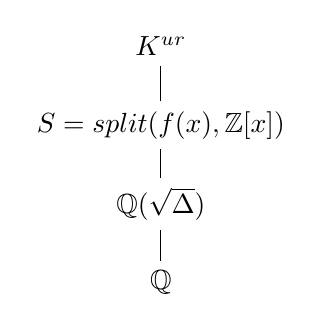
\begin{tikzpicture}[node distance = 1cm, auto]
      \node (Q) {$\mathbb{Q}$};
      \node (K) [above of=Q] {$\mathbb{Q}(\sqrt{\Delta})$};
      \node (S) [above of=K] {$S=split(f(x),\mathbb{Z}[x])$};
      \node (Kur) [above of=S] {$K^{ur}$};
      \draw [-] (K) to node {} (S);
      \draw [-] (Q) to node {} (K);
      \draw [-] (S) to node {} (Kur);
      \end{tikzpicture}
\end{center}
\newline
Using Cohn(1955) and verifying with computer search we calculate that a quintic polynomial that satisfies the above conditions, and has minimal absolute discriminant is $f(x) = x^5-2x^3-x^2+1$ which has $\Delta(f) = -4511\equiv1 (mod 4)$.
This polynomial has root discriminant = 67.16.
Using the bounds in given in Table(2) of Odlyzko(1990) we find that indeed $K^{ur}\cong A_{5}$. 

%% The Appendices part is started with the command \appendix;
%% appendix sections are then done as normal sections
%% \appendix

\begin{thebibliography}{9}
\title{References}
\bibitem{HOEL} 
Long Hoelscher, Jing, \textit{Galois extensions ramified at one prime} (2007). Dissertations available from ProQuest. AAI3260949. 
\bibitem{JONE} 
Jones J.W., Roberts D.P. (2008) \textit{Number Fields Ramified at One Prime}. In: van der Poorten A.J., Stein A. (eds) Algorithmic Number Theory. ANTS 2008. Lecture Notes in Computer Science, vol 5011. Springer, Berlin, Heidelberg
\bibitem{KIM1}
Kim, Kwang-Seob. \textit{Construction of unramified extensions with a prescribed Galois group}. Osaka J. Math. 52 (2015), no. 4, 1039--1051. https://projecteuclid.org/euclid.ojm/1447856031
\bibitem{MAIR}
Maire, Christian. (2006). \textit{On infinite unramified extensions. Pacific Journal of Mathematics}. 192. 10.2140/pjm.2000.192.135. 
\bibitem{ODL1}
Odlyzko, A. M. \textit{Bounds for discriminants and related estimates for class numbers, regulators and zeros of zeta functions : a survey of recent results}. Journal de théorie des nombres de Bordeaux, Volume 2 (1990) no. 1, pp. 119-141. 
\bibitem{ODL2}
Odlyzko, A. M. \texit{Lower bounds for discriminants of number fields}, II. Tohoku Math. J. (2) 29 (1977), no. 2, 209--216. doi:10.2748/tmj/1178240652. https://projecteuclid.org/euclid.tmj/1178240652
\bibitem{KIM2}
Kim, Kwang-Seob & Koenig, Joachim. (2017). Some examples of quadratic fields with finite nonsolvable maximal unramified extensions II. The Ramanujan Journal. 10.1007/s11139-018-0046-3. 
\bibitem{YAMA}
Yamamoto, Yoshihiko. On unramified Galois extensions of quadratic number fields. Osaka J. Math. 7 (1970), no. 1, 57--76. https://projecteuclid.org/euclid.ojm/1200692686
\bibitem{BRIN}
Brink, David. (2010). Remark on infinite unramified extensions of number fields with class number one. Journal of Number Theory - J NUMBER THEOR. 130. 304-306. 10.1016/j.jnt.2009.08.013. 
\end{thebibliography}

\end{document}

